\chapter{Web Services Description Language}

For Web Services, the mere communication, as for instance we know if from
traditional CGI programming, is not everything. The communication is performed
via the SOAP protocol, and there are several implementations of SOAP on top of
CGI. What the here explained WSDL (Web Services Description Language) is about
is the \textit{talking} about Web Services. In a now standardised XML-based format,
one can emply WSDL to describe both technically and for regular users the
performance of the Web Service.

WSDL may be imagined as a meta language. Beside the
description of the service, WSDL renders the possibility that services can be
discovered by service brokers\footnote{The here referenced brokering is meant
to act on a global registry of services and has little practical meaning. It
is not to be confused with the brokering of grid resources, for which ARC-1
provides a web service on its own, which is a key functionality of any
computational grid.}. The discovery of services may be useful for an automatic
adaption of a running client, i.e. if the endpoint of the service changes or to share the load of demands. The WSDL service specification enables a foreign programmer to implement a suitable client which interfaces the service in a proper way. WSDL describes the structure of the messages, the intended use of the messages, the supported protocols and the endpoint
of the service (URL).
\task{For that last reason, every instance of a service must be produced a
distinct WSDL file for - or - it is automatically prepared from the information
that the server has available once it is implemented. - ??MG }\\

WSDL documents are composed of five main elements:
\newcommand{\parboxWidth}{13cm}
\begin{itemize}
	\item \textbf{Types} --- The element \textit{types} contains the description of the message structures and is written in the language XSD (XML Schema Definition). The data types used for the messages of the Echo Web Service are defined starting with the  line~\ref{lst_code:echo_wsdl_types}.

	\item \textbf{Message} --- Within the element \textit{message} a subset of the previously defined types are assigned to be a message. In case of the Echo Web Service  two messages are designated: echoRequest and echoResponse, compare lines line~\ref{lst_code:echo_wsdl_message1} and \ref{lst_code:echo_wsdl_message2}.

	\item \textbf{Port type} --- The element \textit{portType} is used to assign the messages to an interface. Four interface types can be distinguished: One-way (input), request-response (input, output), solicit-response (input, output, fault) and notification (output).
	The Echo Web Service realises a solicit-response interface which is declared subsequent to line~\ref{lst_code:echo_wsdl_portType}. % in the lines followed by the line X

	\item \textbf{Binding} --- The protocol and the data format used for the message transmission are denoted in the element \textit{binding}. Possible style attributes are \textit{document} or \textit{rpc} (Remote Procedure Call). The transport attribute defines the protocol which is regularly HTTP. For each operation a corresponding SOAP action has to be defined which assignes a messages to be either \textit{literal} or \textit{encoded}~\cite{BUTEK_2009}. The service implemented in this chapter will use the binding \textit{document}/\textit{literal} and the protocol HTTP which is to be seen in the lines follow line~\ref{lst_code:echo_wsdl_binding}.

% The style attribute can be "rpc" or "document". In this case we use document. The transport attribute defines the SOAP protocol to use. In this case we use HTTP.
%The operation element defines each operation that the port exposes.
%For each operation the corresponding SOAP action has to be defined. You must also specify how the input and output are encoded. In this case we use "literal".
%  http://www.ibm.com/developerworks/webservices/library/ws-whichwsdl/
%   1. RPC/encoded    (Remote Procedure Call)
%   2. RPC/literal
%   3. Document/encoded
%   4. Document/literal
% The terminology here is very unfortunate: RPC versus document. These terms imply that the RPC style should be used for RPC programming models and that the document style should be used for document or messaging programming models. That is not the case at all. The style has nothing to do with a programming model. It merely dictates how to translate a WSDL binding to a SOAP message. Nothing more. You can use either style with any programming model.
%
% RPC/literal SOAP message for myMethod
%
%<soap:envelope>
%    <soap:body>
%        <myMethod>
%            <x>5</x>
%            <y>5.0</y>
%        </myMethod>
%    </soap:body>
%</soap:envelope>
%
%  RPC/encoded SOAP message for myMethod
% 
% <soap:envelope>
%     <soap:body>
%         <myMethod>
%             <x xsi:type="xsd:int">5</x>
%             <y xsi:type="xsd:float">5.0</y>
%         </myMethod>
%     </soap:body>
% </soap:envelope>

	\item \textbf{Service} --- Within the last WSDL element \textit{service} the
	endpoint of the service gets specified. As to be seen in
	line~\ref{lst_code:echo_wsdl_service} the endpoint of the Echo Web Service is
	assigned to \textit{http://localhost:60000/echo}.
\end{itemize}

To understand an WSDL document, one best starts from the Service entry,
commonly located at the end. It will describe what the service is all about.
From there, move upwards to learn about the operations and their parameters.
Most items in the WSDL document have their own tags that provide names or
descriptions.
%\textcolor{white}{newline}
\lstsetJUSTXML
\lstinputlisting
	[
	label=lst:echo_wsdl,
	caption={[WSDL file describing the echo service. Filename: echo.wsdl]
	\textbf{WSDL file describing the echo service. Filename: echo.wsdl}}
	]
{../src/services/echoservice/echo.wsdl}
\task{TODO: Validate the WSDL Listing}

\section{How to prepare a WSDL document}

It should be said that the preparation of WSDL documents not ultimate fun to
do. And it is tricky in the sense that one does mistakes easily that are
difficult to spot.

The community hence started to use computational tools to draft these documents.
The most prominent of these is probably Eclipse. Since its version 3.4 (you
might need to install it directly from \url{http://www.eclipse.org} if your
distribution is a bit behind or if you are working with Windows) it offers a
web tools platform (WTP) module with which WSDL files can be crafted graphically.
To install it, point the url http://download.eclipse.org/webtools/updates/ to
the Eclipse updater, if it is not already listed.

\subsection{Preparation of the Echo WSDL file with Eclipse}

\begin{figure}
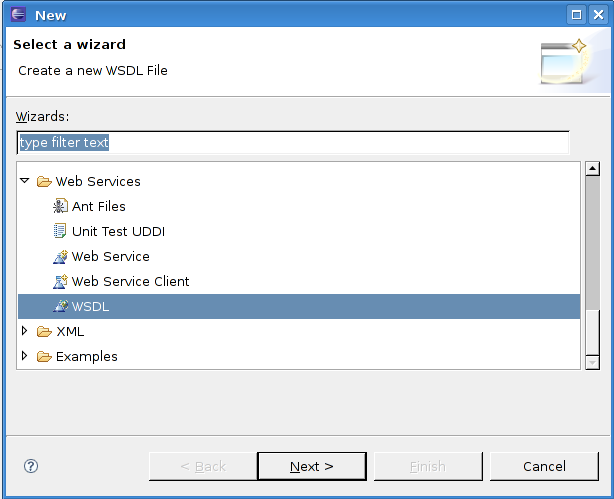
\includegraphics[width=.4\columnwidth]{tex_wsdl/wsdl_NewFileMenu.png}
\caption{Eclipse dialog to create a new file. WSDL is selected.}
\label{fig:wsdl_newFileMenu}
\end{figure}

To prepare a WSDL document with Eclipse, one should find the right file type in
the typical Eclipse dialog window. This is shown in figure
\ref{fig:wsdl_newFileMenu}. The empty WSDL document is not empty, but the
application starts with a minimal setup: a service that expects some input and
provides some immediate return value. This is already much like the echo web
service. One basically only needs to add the documentation of the service and
to name the parameters. To do so, just click on the items displayed in the
graphical representation and/or find respective entries in the tabs below.

\begin{figure}
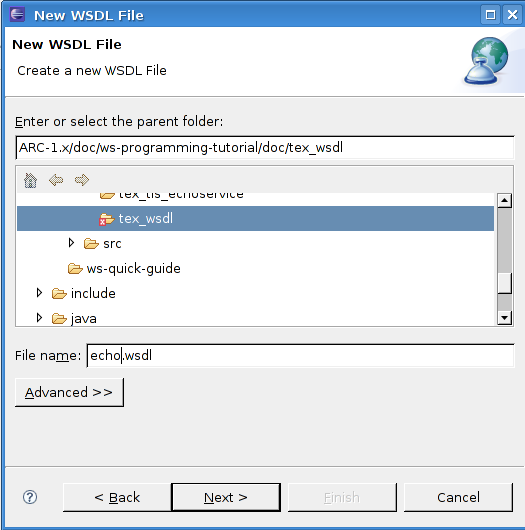
\includegraphics[width=.4\columnwidth]{tex_wsdl/wsdl_NewWSDLfile.png}
\caption{The default settings are fine for a WSDL service that communicates
with ARC.}
\end{figure}

\begin{figure}
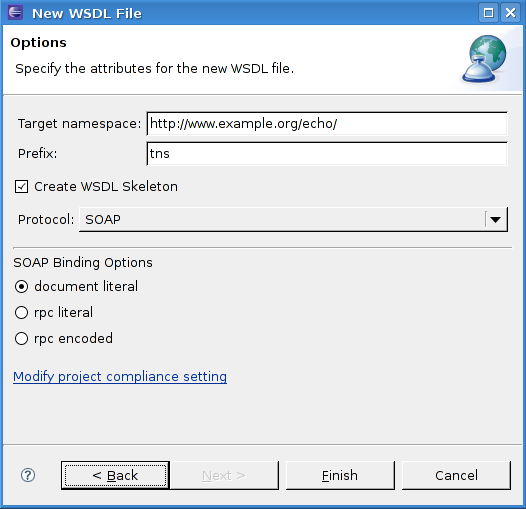
\includegraphics[width=.4\columnwidth]{tex_wsdl/wsdl_defaultSettings.png}
\caption{The project first shown has already a strong similarity to the Echo
web service that is planned for.}
\end{figure}

\begin{figure}
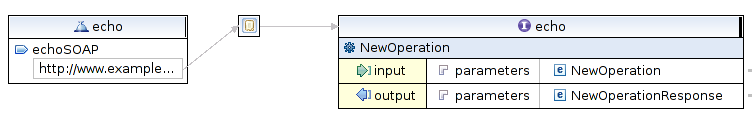
\includegraphics[width=.4\columnwidth]{tex_wsdl/wsdl_defaultProject.png}
\caption{A first usable web service description is achieved solely by
specifying the address and passing the arguments the known type
\textit{string}.}
\end{figure}

\begin{figure}
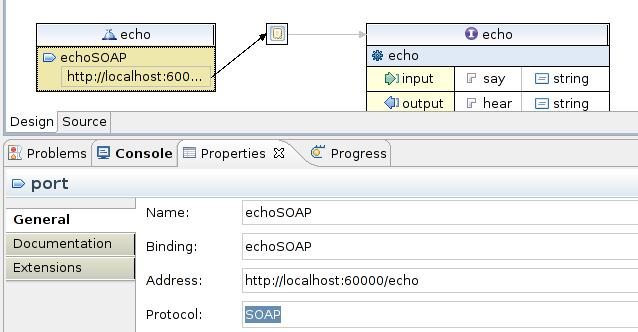
\includegraphics[width=.4\columnwidth]{tex_wsdl/wsdl_EchoSimplest.png}
\caption{The WSDL for echo in a very simplistic manner.}
\label{fig:simpleEchoService}
\end{figure}

\subsection{Inspection of Web Services with Taverna}

One will fine many specifications that are needed by WSDL to glue the different
parts of the WSDL file together. The service references the bindings and the
bindings reference the port and so on. One should not become overly nervous
about it. The regular programmer does not see those internal names. A good
sanity check for the programmer's view on a WSDL file is to load it from within
the workflow suite Taverna\footnote{Taverna is available from
\url{http://taverna.sf.net}. ARC offers a plugin that allows the direct
communication of Taverna with resources runnign ARC-0. An interface to ARC-1
is still pending. In principle, there is none needed. In practice, we still need
more practice to decide.}.

\begin{figure}
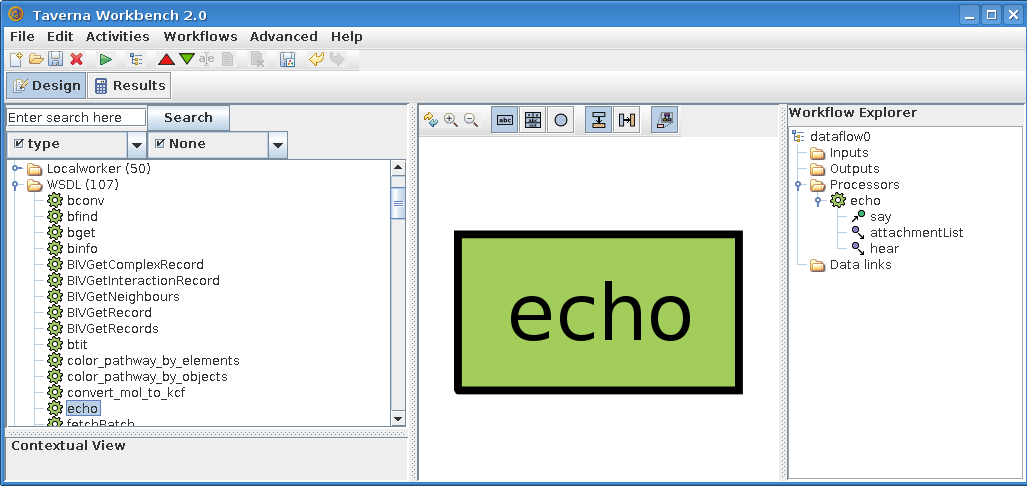
\includegraphics[width=.7\columnwidth]{tex_wsdl/wsdl_echo_taverna_minimal.png}
\caption{Taverna learned about the Echo Web Service and presents it. No
internal names of WSDL appear, only the name of operations and paramters are
shown.}
\label{fig:wsdlEchoTavernaMinimal}
\end{figure}

The \textit{activities} menu in Taverna offers the item \textit{New Activity}.
It will request the specification of an URL or a local path that points to a
WSDL file. The services presented in there will then be added to the list of
WSDL resources. So will the \textit{echo} workflow that was just prepared with
Eclipse. When it is dragged to the canvas in the middle, as shown in figure
\ref{fig:wsdlEchoTavernaMinimal}, it appears as an interactive object. To the
right, the parameters of the operation are displayed.

\begin{figure}
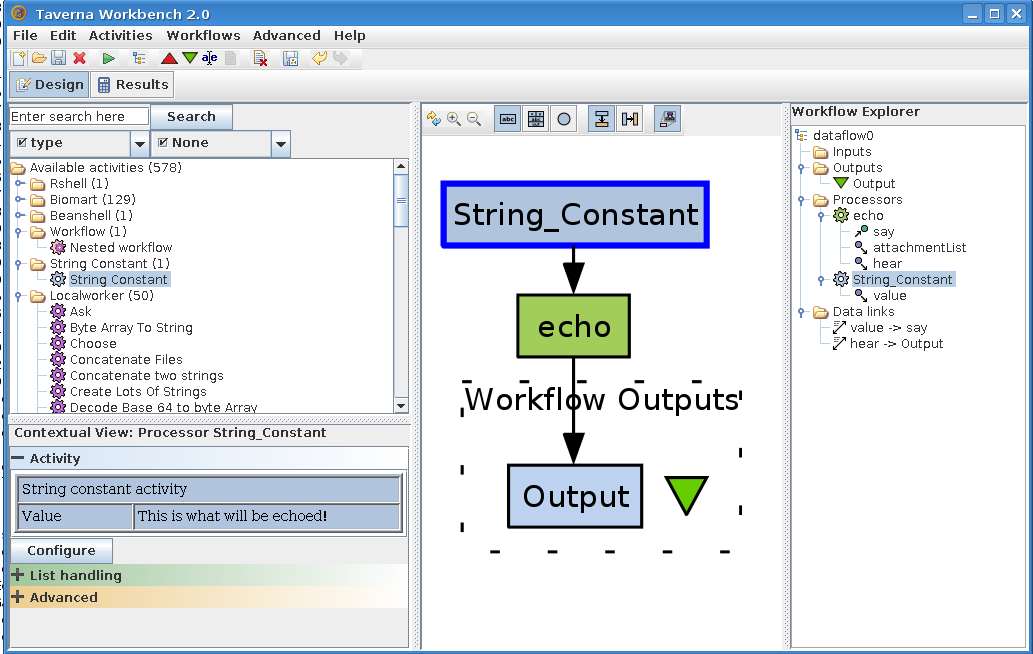
\includegraphics[width=.7\columnwidth]{tex_wsdl/wsdl_echo_taverna_context.png}
\caption{A completely functional (albeit small) workflow in Taverna that
addresses the Echo Web Service prepared with HED.}
\label{fig:wsdlEchoTavernaContext}
\end{figure}

With a string constant as a constant input added, alternatively one could link a
configurable workflow input as input to the echo Web Service, and the
workflow's output linked as a sink to the output of the workflow, the workflow
is complete. It can now be executed, presuming that the localhost is indeed
running arched with the echo service as described in section
\ref{sec:arch_echo_web_service}.

When comparing the GUI representation of Eclipse as shown with in figure
\ref{fig:simpleEchoService} or that of the just shown Taverna representation
with the raw WSDL of listing \ref{lst:wsdl_eclipse_echo_xml}, it becomes
apparent, that the raw form of the WSDL, as shown below, is more complicated. It seems to invent nested structures that are just not present, since it is only simple strings that are exchanged.
The good news here is, that one would have reached exactly that more
complicated looks when following the original setup without assignment of the
simple type 'string'. WSDL needs special types for every operation. And eclipse
provides them, even when the input types are shown in a more simple manner.


\lstsetECHOECLIPSEXML
\lstinputlisting
	[label=lst:wsdl_eclipse_echo_xml,float=htb,
	caption={[Minimalistic WSDL file for echo created with Eclipse.]
	\textbf{WSDL file for Echo created with Eclipse.}}]
{tex_wsdl/echo.wsdl}

This has the advantage, that you can use this WSDL file to describe the regular
ARC echo service, even though the original programmer might not have used
Eclipse to create it. Or has he? Gabor?


\section{What else to do with WSDL}

There are several efforts to organise the world of web services and their
interactions. Taverna was already mentioned above. Amongst the most advanced
scientific community with respect to Web Services are the Bioinformaticians.
Topics that come to mind are:

\begin{itemize}
  \item BioMoby \url{www.biomoby.org}
  \item $^my$Grid and $^my$Experiment \url{www.myexperiment.org}
  \item Distributed Annotation System (DAS) \url{http://www.biodas.org} 
\end{itemize}

But this is left for a future version of this tutorial\ldots and/or possibly
Hajo's Bachelor thesis.



